\documentclass[a4paper,10pt]{article}
\usepackage[top=1.0in, bottom=1.0in, left=1.0in, right=1.0in]{geometry}
\usepackage[utf8]{inputenc}
\usepackage{graphicx}
\usepackage{float}
\usepackage{subfig}
\usepackage[square,numbers]{natbib}
\bibliographystyle{unsrtnat}

\title{EEC 289A - Project \\ Reinforcement Learning for Remeshing}
\author{Ahmed H. Mahmoud}
\date{} 
\begin{document}

\maketitle

\section{Abstract:}
In this work, we try to improve upon the work represented in ~\citep{Abdelkader:2017:ACR} to add another layer of fine-grained control of the selection of the meshing operator used to enhance the quality of triangular mesh. It has been previous shown that a generic framework can be devised to improve various quality of initial mesh; a process that is important for many computer graphics and simulation applications. The framework consisted of a set mesh operators that can be applied in varying order to the input initial mesh. However, there is no consistent scheduling of such operators and it was left to the user to choose the right scheduling. In this report, we argue that it is possible to automate the scheduling by leveraging ideas from reinforcement learning and integrate it in the framework. Doing so, it is possible to apply the framework on large set of quality that no mapping into geometric primitives e.g., aligning mesh edges with an underlying directional field ~\cite{Jakob:2015:IFM:2816795.2818078}. 


\section{Introduction:}
Processing of geometric models is a common practice in computer graphics ~\citep{Alliez2008}, visualization, finite element analysis for simulation ~\citep{ho1988finite}, and computer aided-design. These models are used as linear approximation for some underlying surface. These models or meshes could be acquired by laser scanner or modeling tool such as Autodesk Maya, ZBrush or Blender. Such process usually produces noisy meshes with artifacts that makes the processing of such meshes impossible. For that reason, geometry processing comes as an important stage in the 3D modeling acquisition pipeline ~\citep{CGF:CGF00574} to improve the quality of the mesh and make the further processing of the models feasible. Improving the quality of initial mesh is also called \emph{remeshing}.

Remeshing is a multi-objective optimization process where the objective requirement could be sometimes conflicting. That could be the reason why most of the existing remeshing techniques usually focus on one objective. However, there have been a rise on remeshing algorithms with multiple objectives ~\citep{7756294, field, Jakob:2015:IFM:2816795.2818078}. 


The main remeshing objective we will focus on in this work is the non-obtuse of triangular meshes. Non-obtuse remeshing takes input mesh contains triangles with angles larger than $90^{\circ}$ and returns an output mesh with all angles less than $90^{\circ}$. Non-obtuse meshes are vital for the correctness and convergence of numerical solution e.g., fast marching method ~\citep{yan2016non}. It is been proven lately that it is always possible to obtain a non-obtuse triangulation with a polynomial bound over the number of input vertices ~\citep{Bishop2016}. Despite this theoretical results, there is not any remeshing algorithm with guarantees of producing non-obtuse remeshing. The framework devised in \citep{Abdelkader:2017:ACR} can be considered as the state-of-art of non-obtuse remeshing as shown by empirical results. However, it is possible that the framework get stuck in certain configuration. The solution suggested in the paper is to re-run the algorithm with different random seed. The random seed will affect the decision over what meshing operator to use and on what vertex being used such that the stuck configuration may not be encountered again. This only holds a probabilistic guarantee that may not be encountered for different models or may need a large number of experiments. 

\paragraph{Contribution:} We propose in this report a way to formulate the problem as reinforcement learning problem i.e., MDP problem. Thus, it is possible to \emph{learn} from previous experiments; and not just re-run the experiment with random seed and wish for better luck. Using this formulation, we experimented with different reinforcement learning algorithms and show that it is possible to guide the algorithm to achieve better results in the next run. 

\section{Remeshing Algorithm:}
We describe here the remeshing framework. The framework is designed to serve various mesh quality or objectives. Since we are only concerned with non-obtuse remeshing, we tailored the framework description to serve the sole purpose of non-obtuse remeshing. The algorithm uses two nested loops; the outer loops is a \emph{while}-loop that keeps repeating the same steps until maximum number of iterations is encountered, and the inner loop iterates over all five remeshing operators (described later). The maximum number of iterations is taken here to be 10. Each remeshing operator is applied on each obtuse angle. All the remeshing operators guarantee to either remesh the obtuse triangle into non-obtuse one or leave it as it is in case of failure. 
\paragraph{Remeshing operators:}
Figure \ref{fig:operators} shows the five operators. We first invest sometime to describe the first operator, \emph{relocation}, and the later operators will be considered as extension of it. 

\begin{enumerate}
\item \textbf{Relocation} is applied on one vertex and seeks to move this vertex such that all triangles share it as a head are non-obtuse. It starts with removing the vertex and all edges connected to it. In order to fill in the void with another vertex and produce non-obtuse triangles, the new vertex should be outside all diameter circles of the edges surrounding the newly created void (shown in red in Figure \ref{fig:operators}(a)). This will prevent any the angle at the head of the vertex (apex) to be non-obtuse. Additionally, in order to prevent the base angle from being obtuse, the new vertex should be one the right side of the two half-planes constructed at the two ends of each edge surrounding the void as shown in Figure \ref{fig:regions}(a). Similar geometric primitives can be constructed in order to prevent the angle from deterioration below certain limit ($\theta_{min}$). Such additional primitives are shown in Figure \ref{fig:regions}(b) while Figure \ref{fig:regions}(c) shows the complete set of geometric primitives used in order to make sure the new vertex is in the region that will guarantee non-obtuse triangles to all triangles connected to the new vertex. Such primitives represent a mapping from the objective function to simple geometric primitives that are easy to construct and work on. Next, we sample the void randomly respecting the feasible region of sampling represented by the geometric primitives. It is possible that the primitives overlap in such a way that no new sample is possible to be drawn inside the void. At such cases, we quit and move to another obtuse triangles. Otherwise, we connect the new vertex to the vertices surrounding the void. 

\item \textbf{Ejection} removes two vertices and add one as shown in Figure \ref{fig:operators}(b). It follows the same steps as for Relocation in terms of constructing the primitives and sampling one vertex. 
\item \textbf{Injection} adds new vertex inside a bad triangles/batch. Here we do not remove any vertices. Instead we remove edges (shown as dotted edges in (Figure \ref{fig:operators}(c)) and this created a void to work on. One or both of the removed edges belongs to an obtuse triangles. The same process of constructing the primitives and sampling one vertex inside the void are followed to produce non-obtuse triangulation. 
\item \textbf{Attractor Ejection:} is an extension to Ejection in which the void vertcies (shown as blue in Figure \ref{fig:operators}(d)) and moved closer to the center of the void. This helps closes up a wide void such that the primitives overlap and a sample can be drawn to produce non-obtuse triangles. 
\item \textbf{Repeller Injection:} is an extension of Injection in which the void vertices are moved away from the center of the void. This could be helpful in widening a tight void and thus a new vertex can be sampled to produce non-obtuse triangles inside the void. 
\end{enumerate}

\begin{figure*}[!tb]
	\centering
	\subfloat[Relocation]{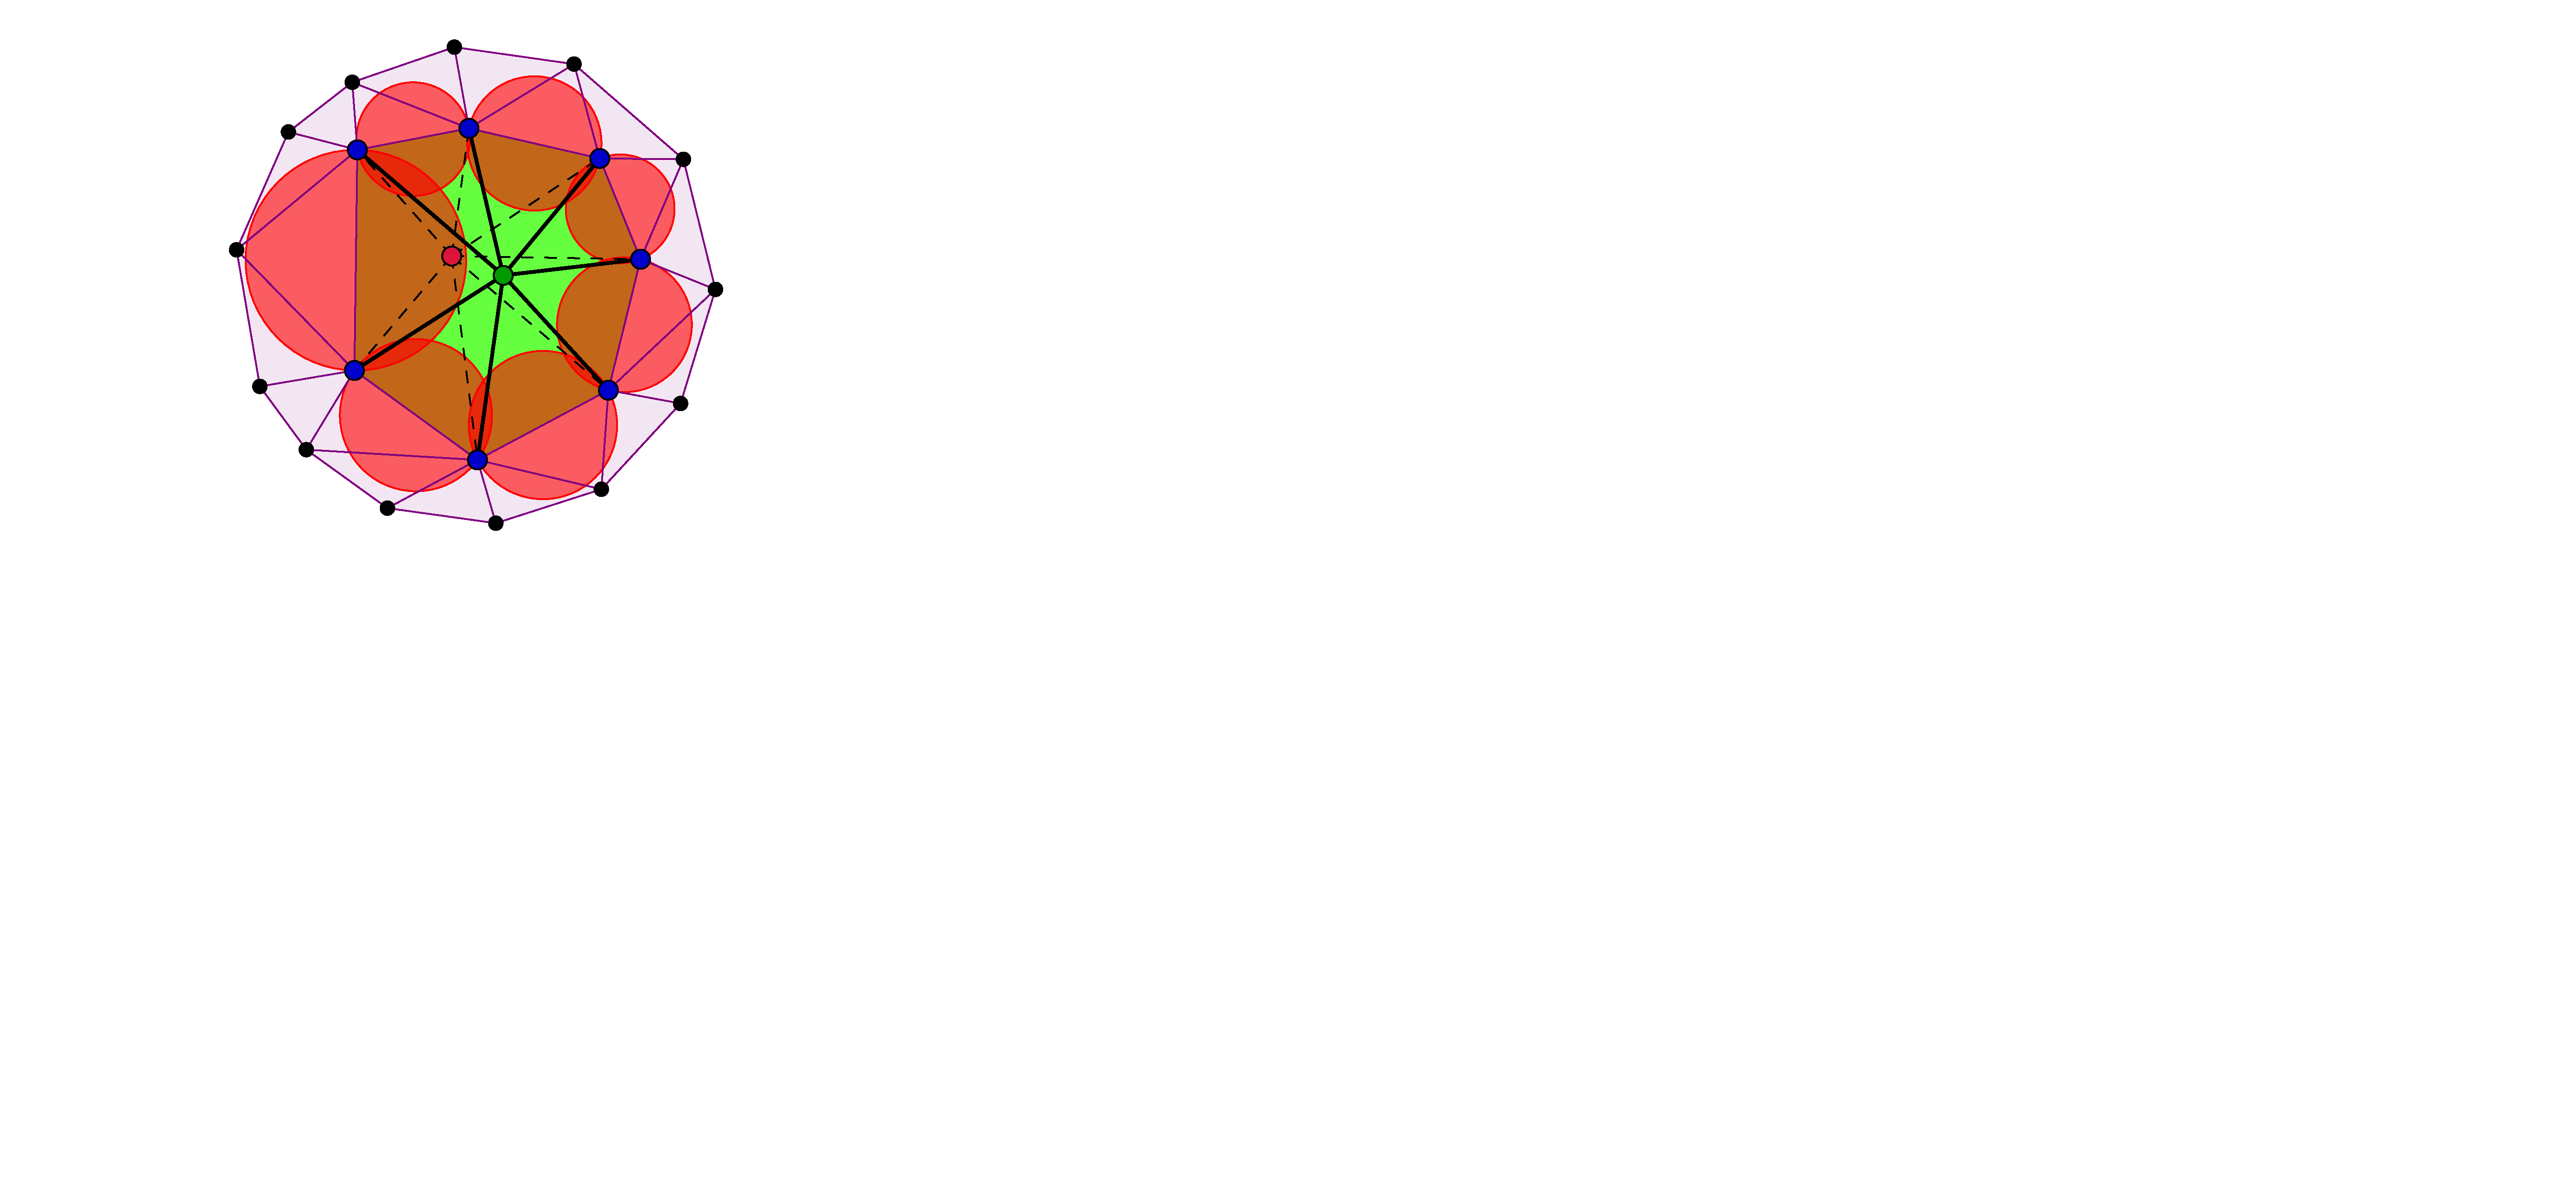
\includegraphics[width=4.0cm,height=4.0cm]{figs/operators/reloc.pdf}}
	\subfloat[Ejection]{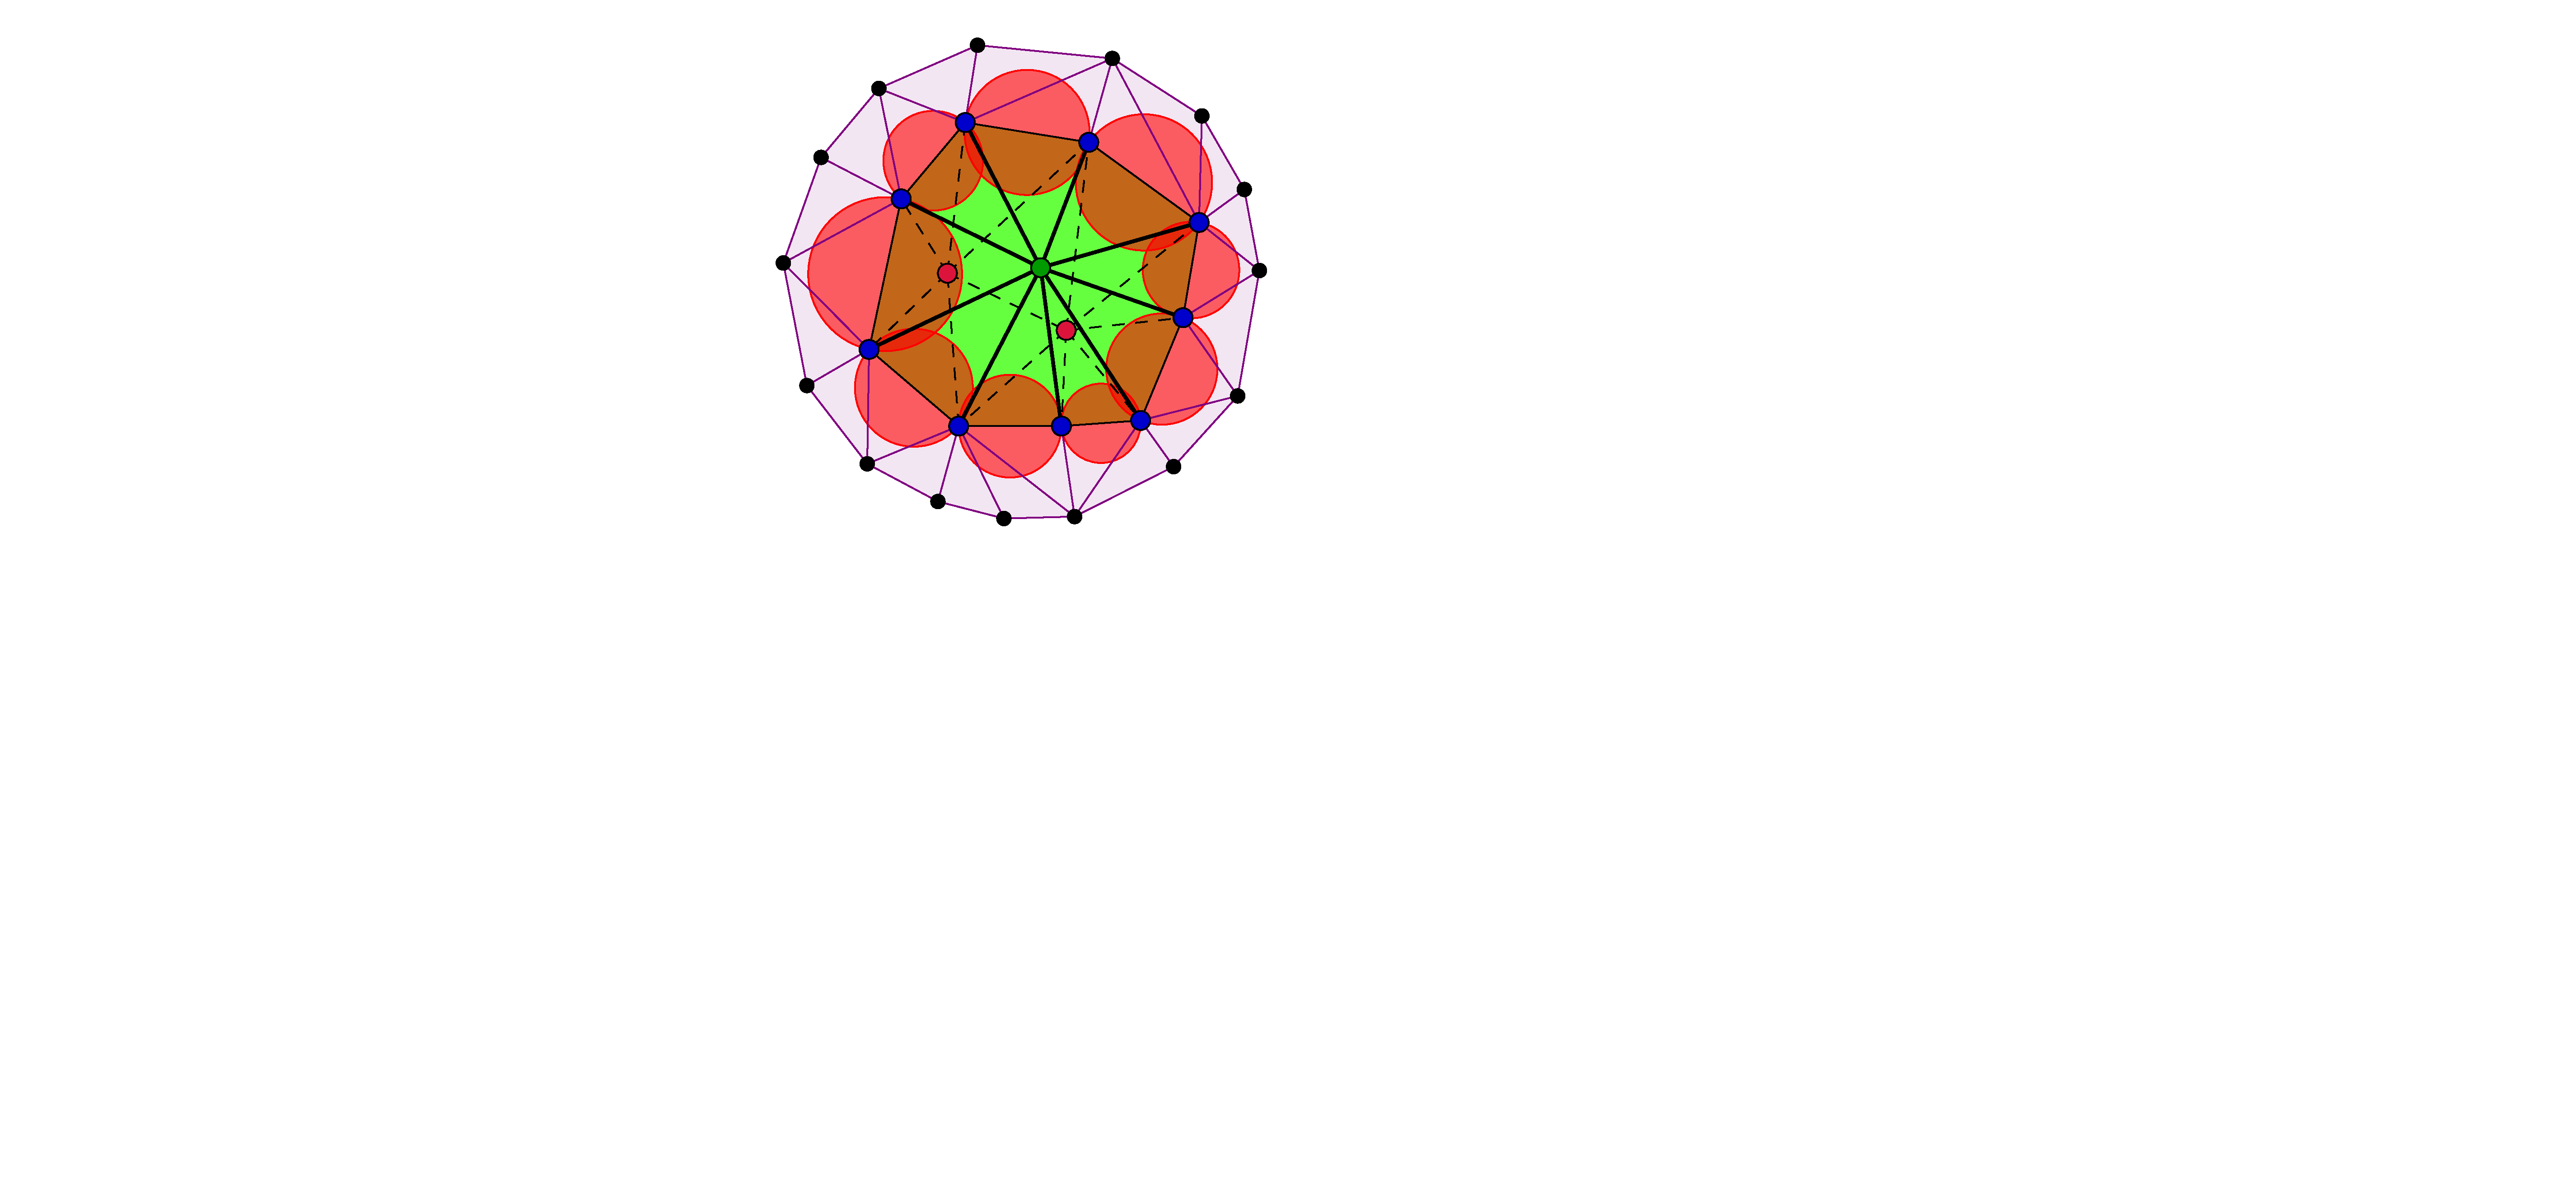
\includegraphics[width=4.0cm,height=4.0cm]{figs/operators/ej.pdf}}	
	\subfloat[Injection]
	{
	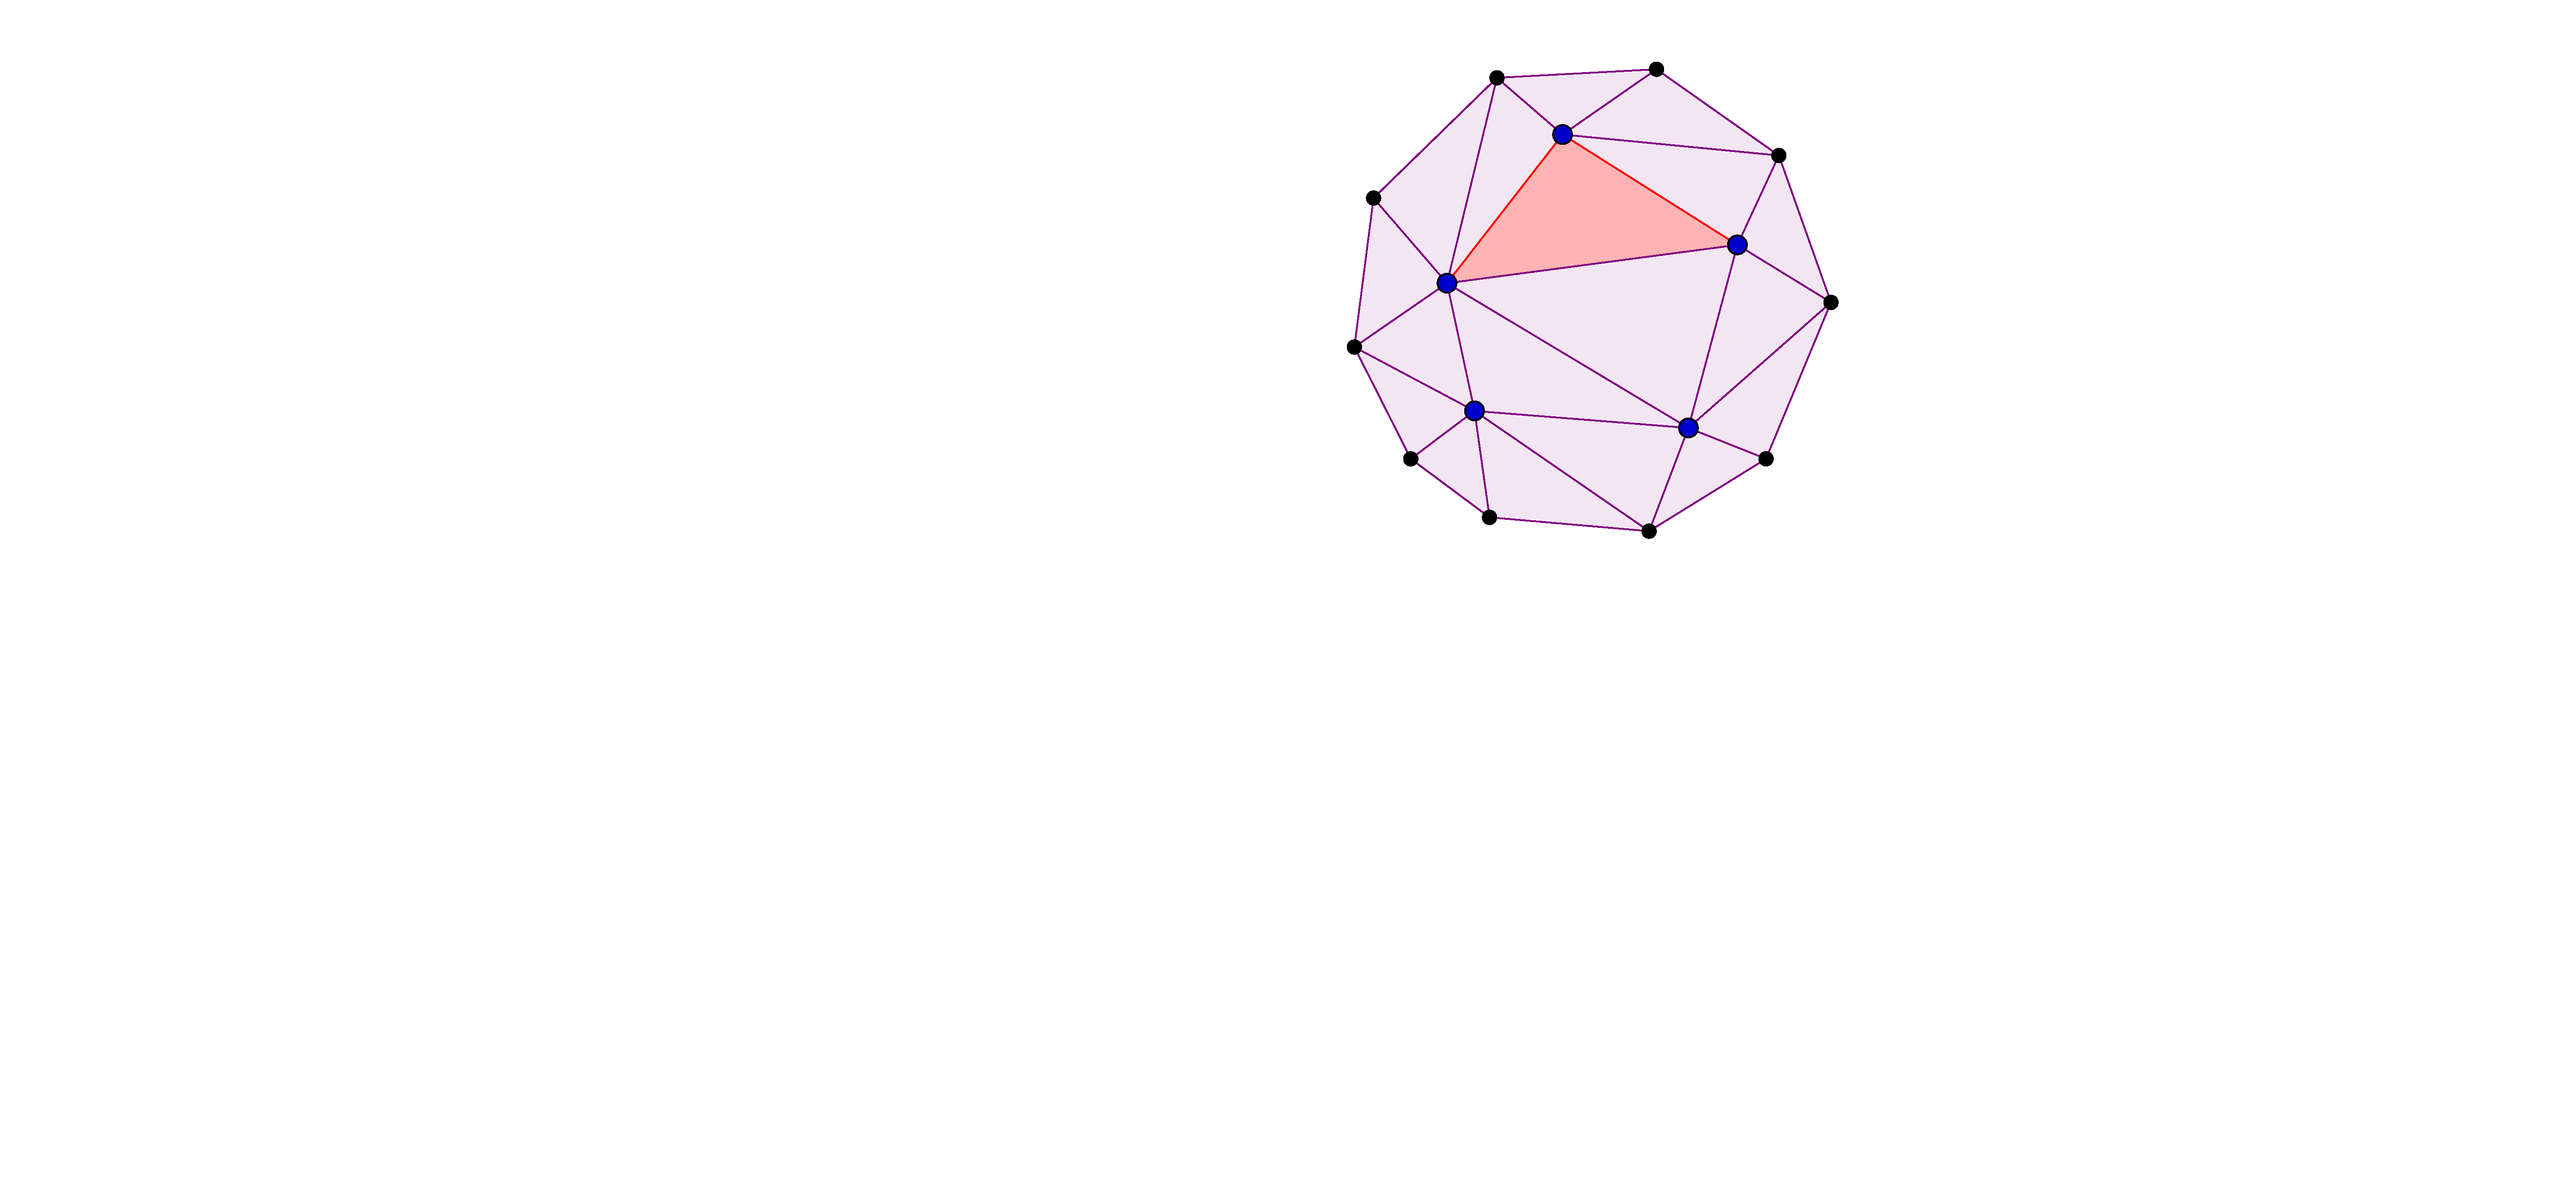
\includegraphics[width=4.0cm,height=4.0cm]{figs/operators/inj_a.pdf}
	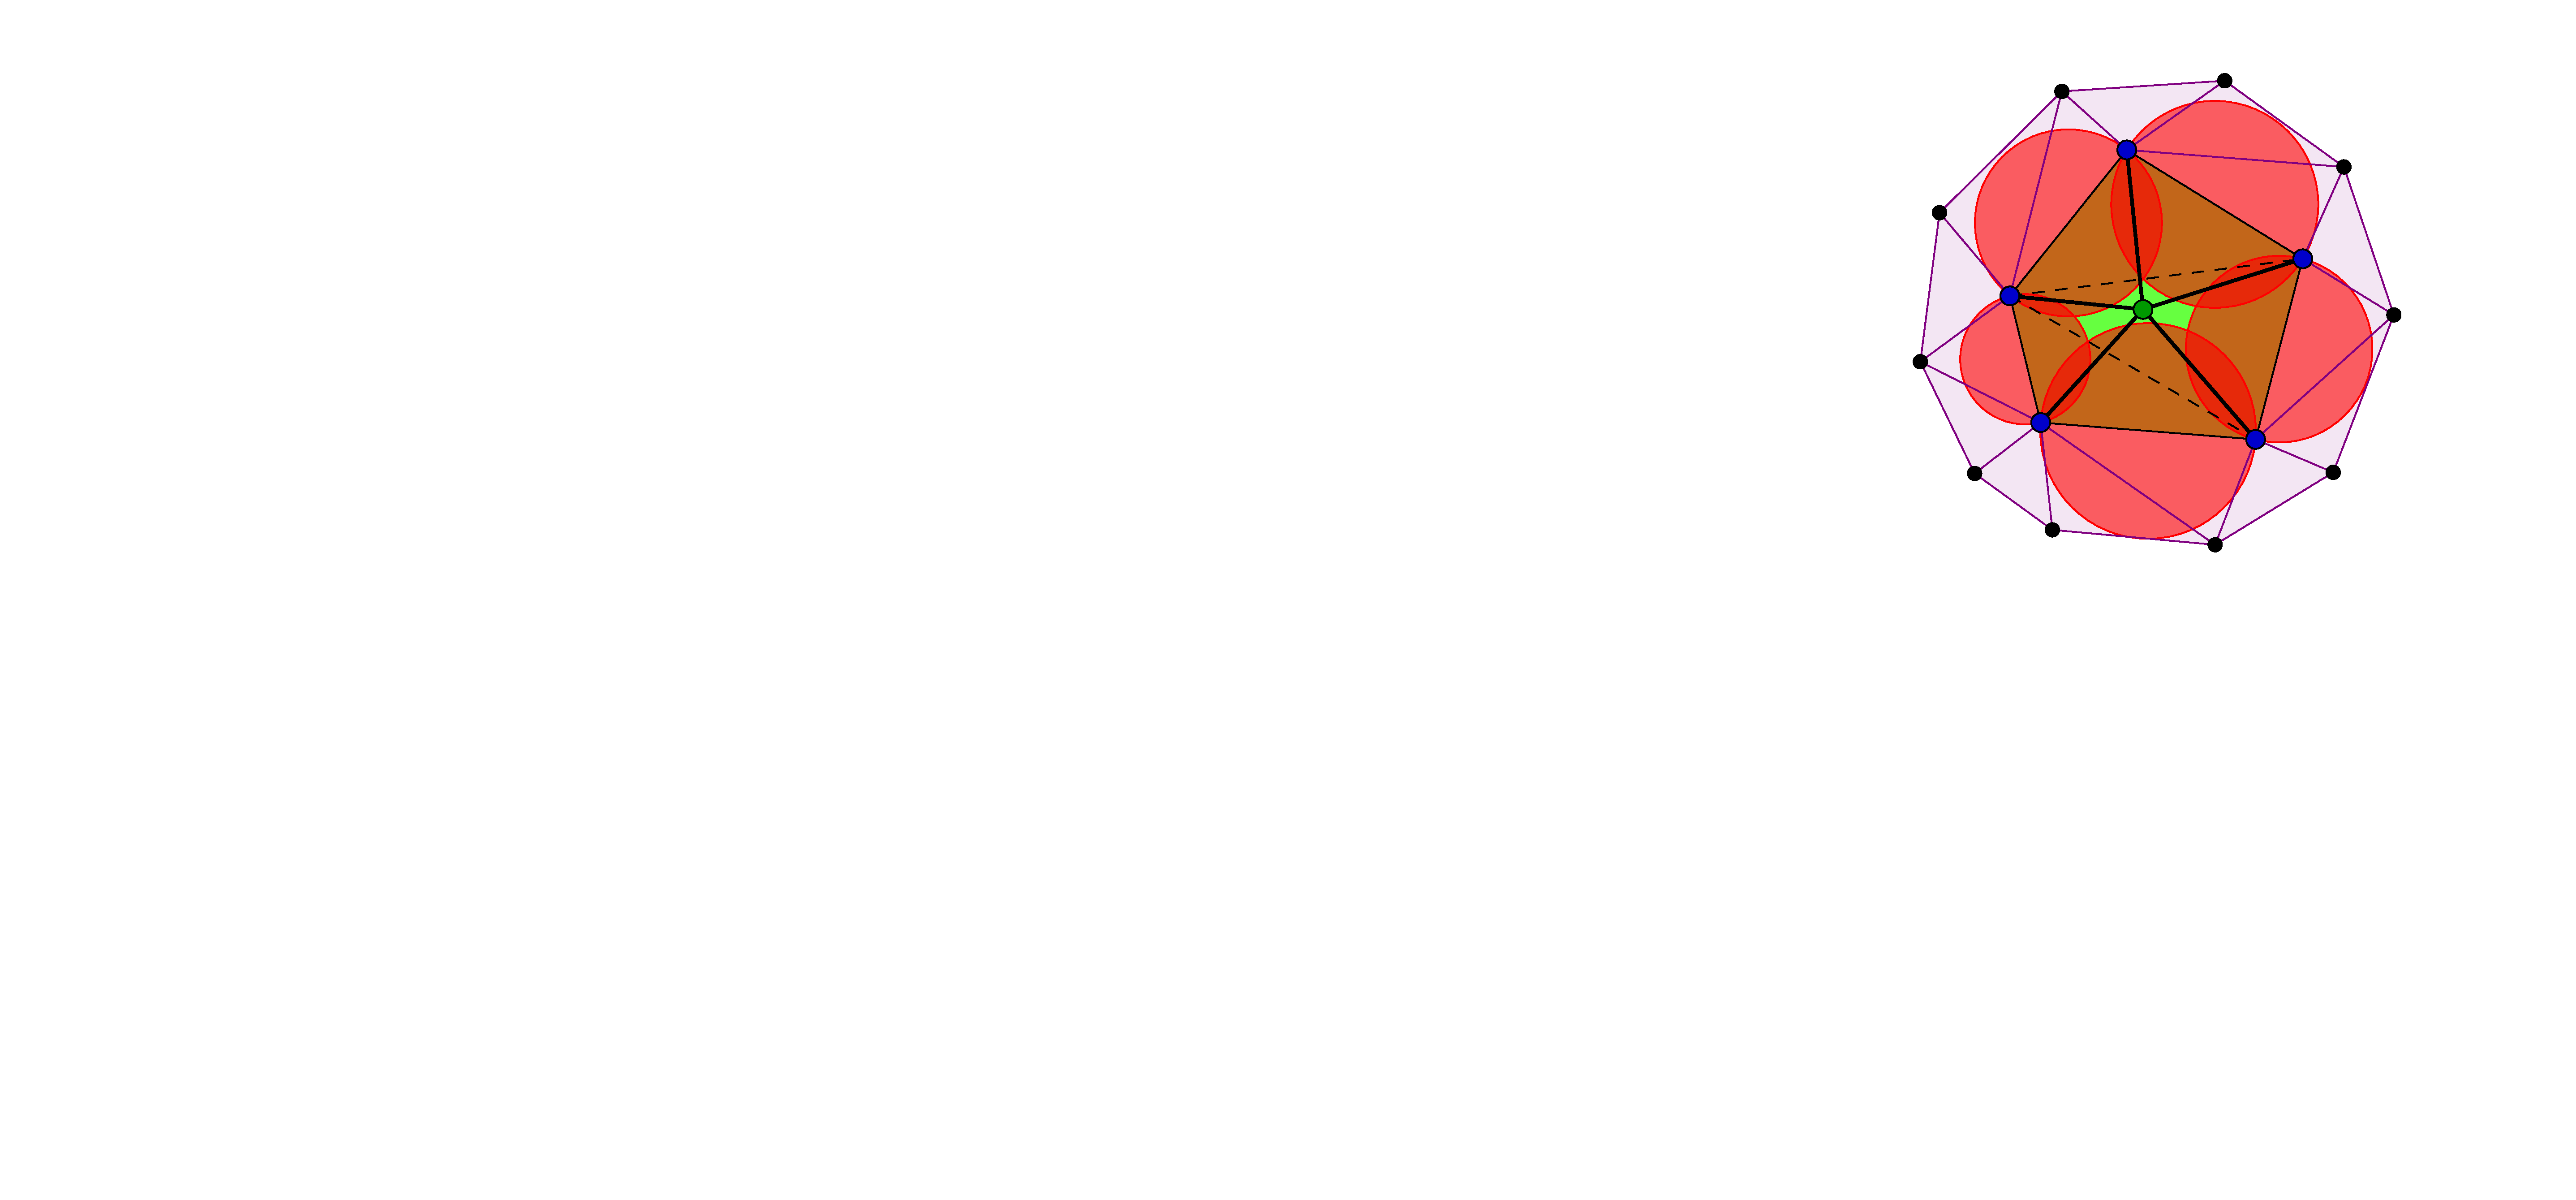
\includegraphics[width=4.0cm,height=4.0cm]{figs/operators/inj_b.pdf}
	}
	
	\subfloat[Attractor Ejection ($\rightarrow$ blue $\leftarrow$)]
	{
	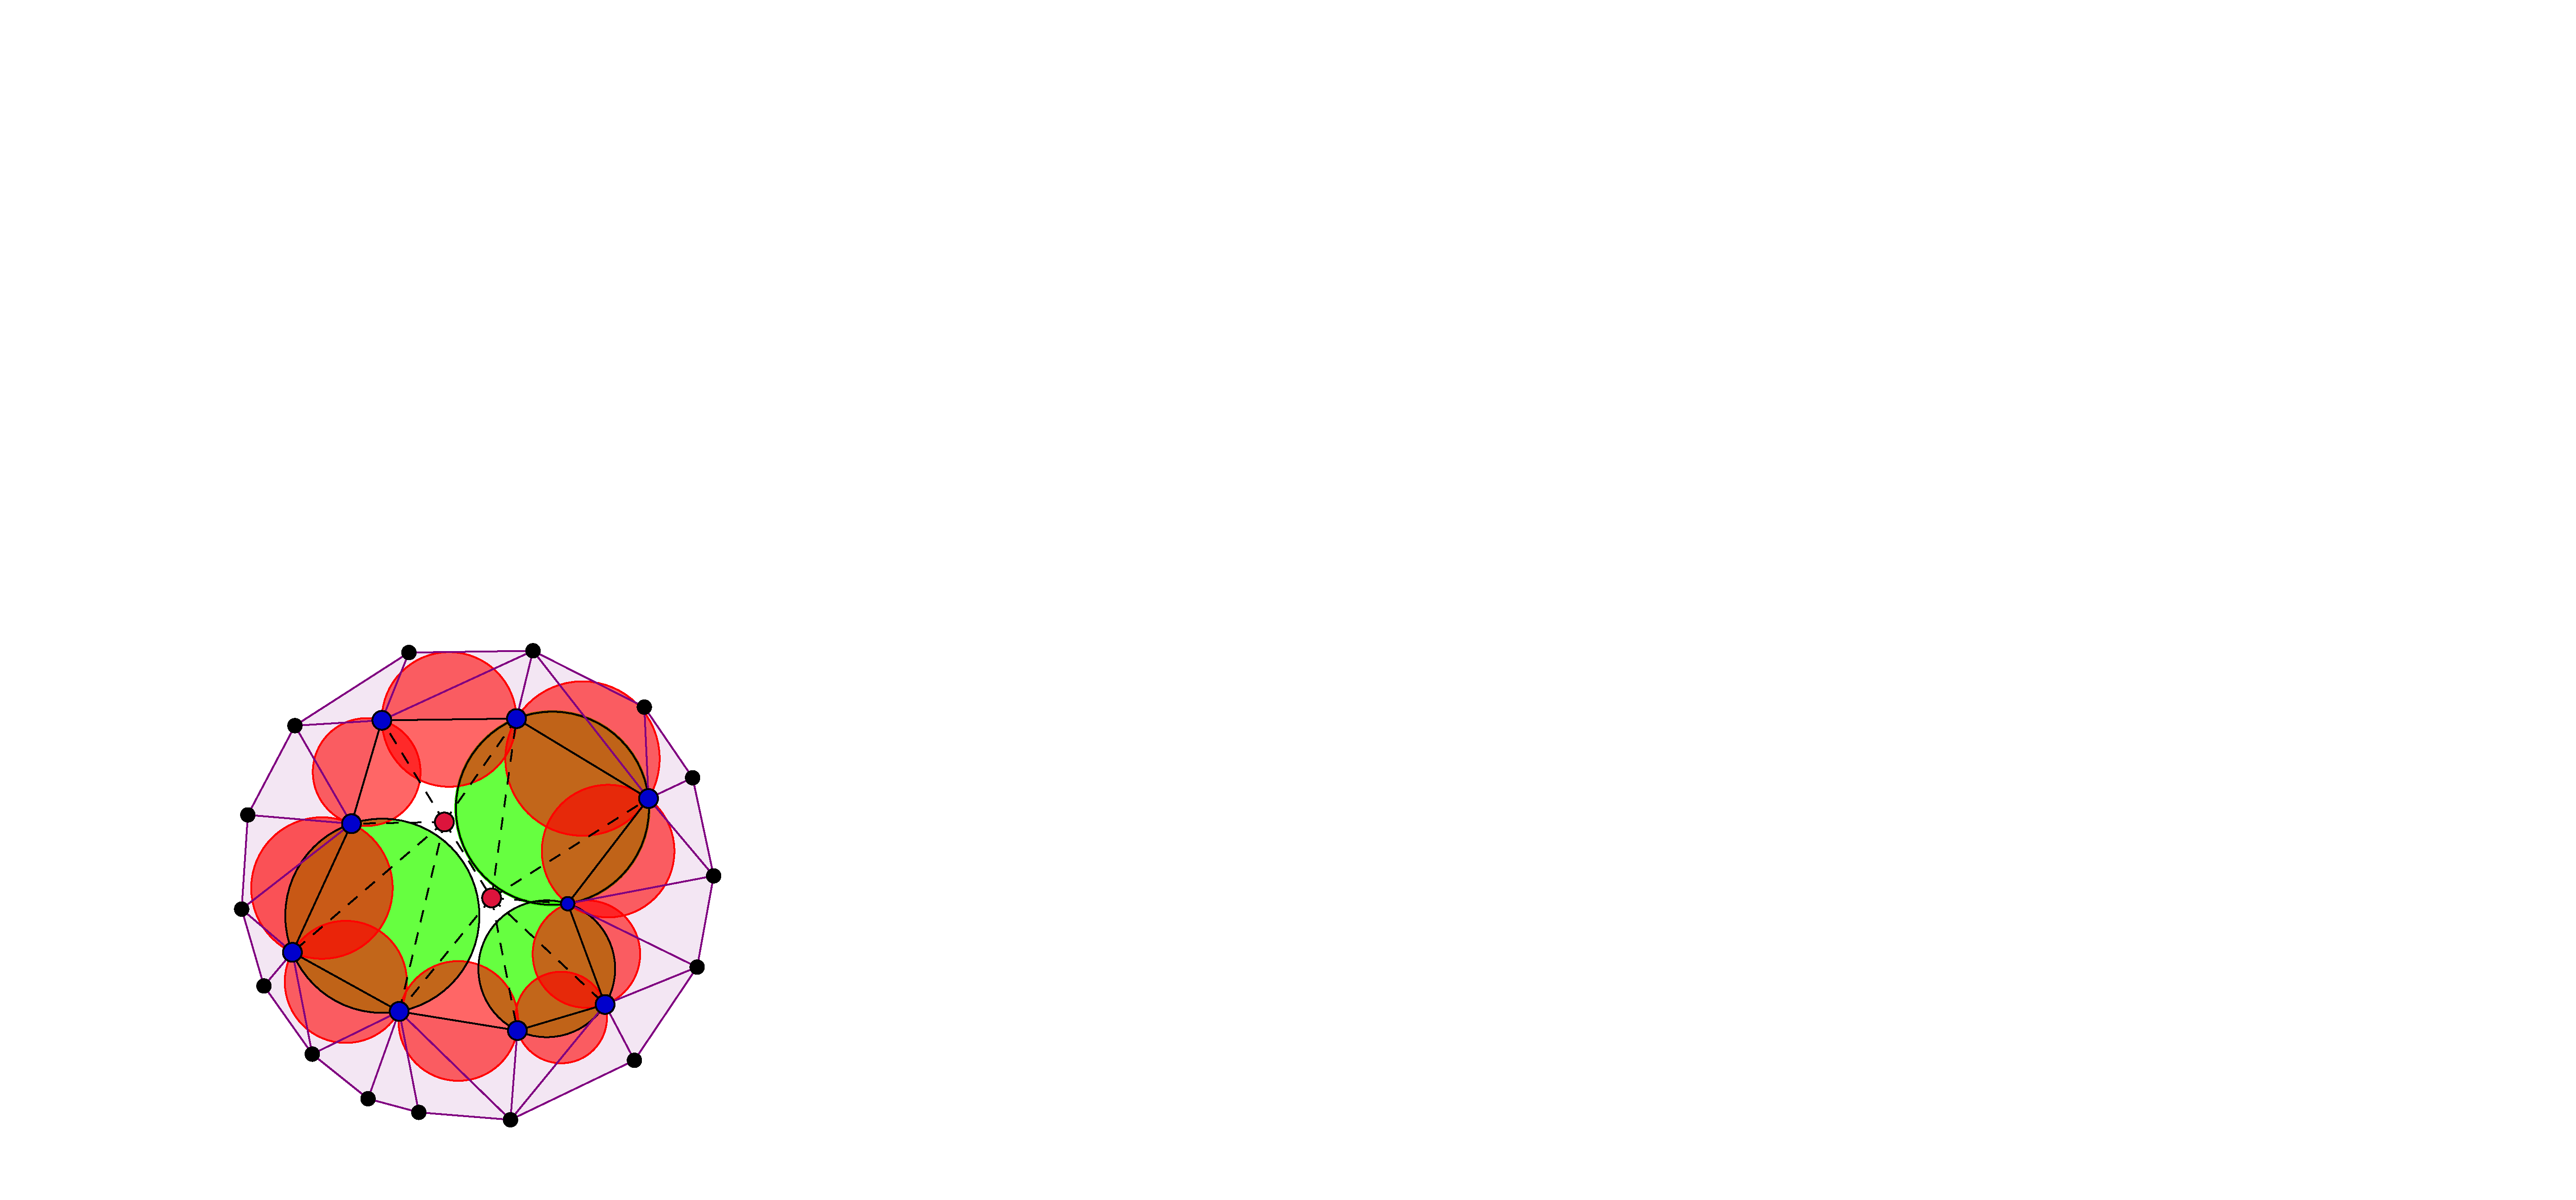
\includegraphics[width=4.0cm,height=4.0cm]{figs/operators/att_a.pdf}
	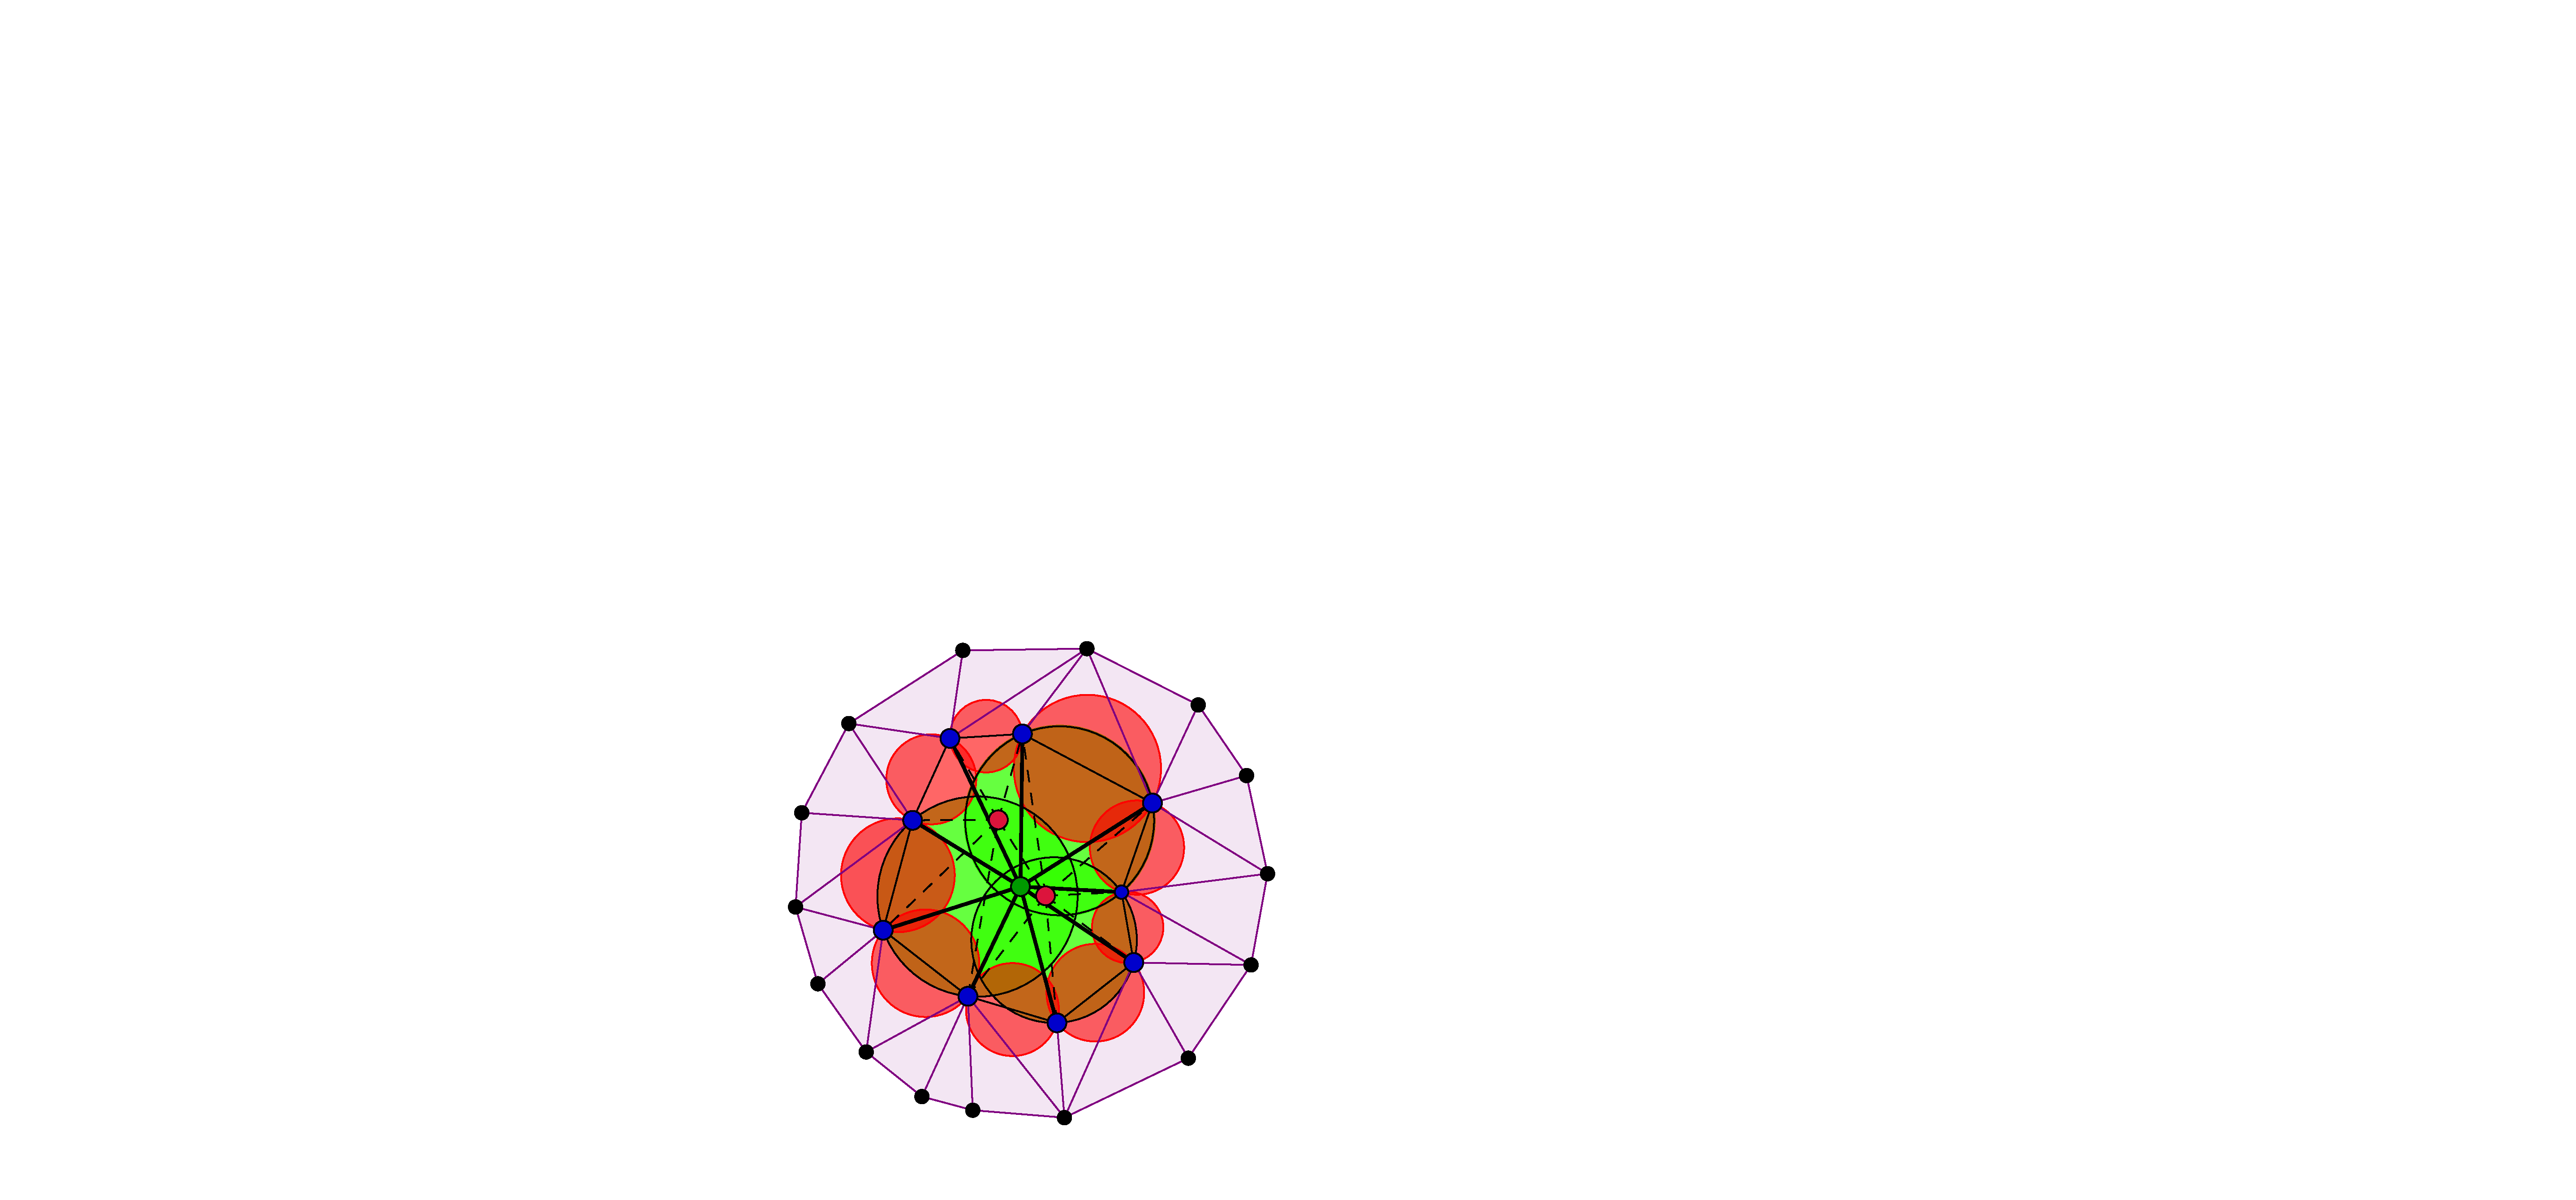
\includegraphics[width=4.0cm,height=4.0cm]{figs/operators/att_b.pdf}	
	}		
	\subfloat[Repeller Injection ($\leftarrow$ blue $\rightarrow$)]
	{
	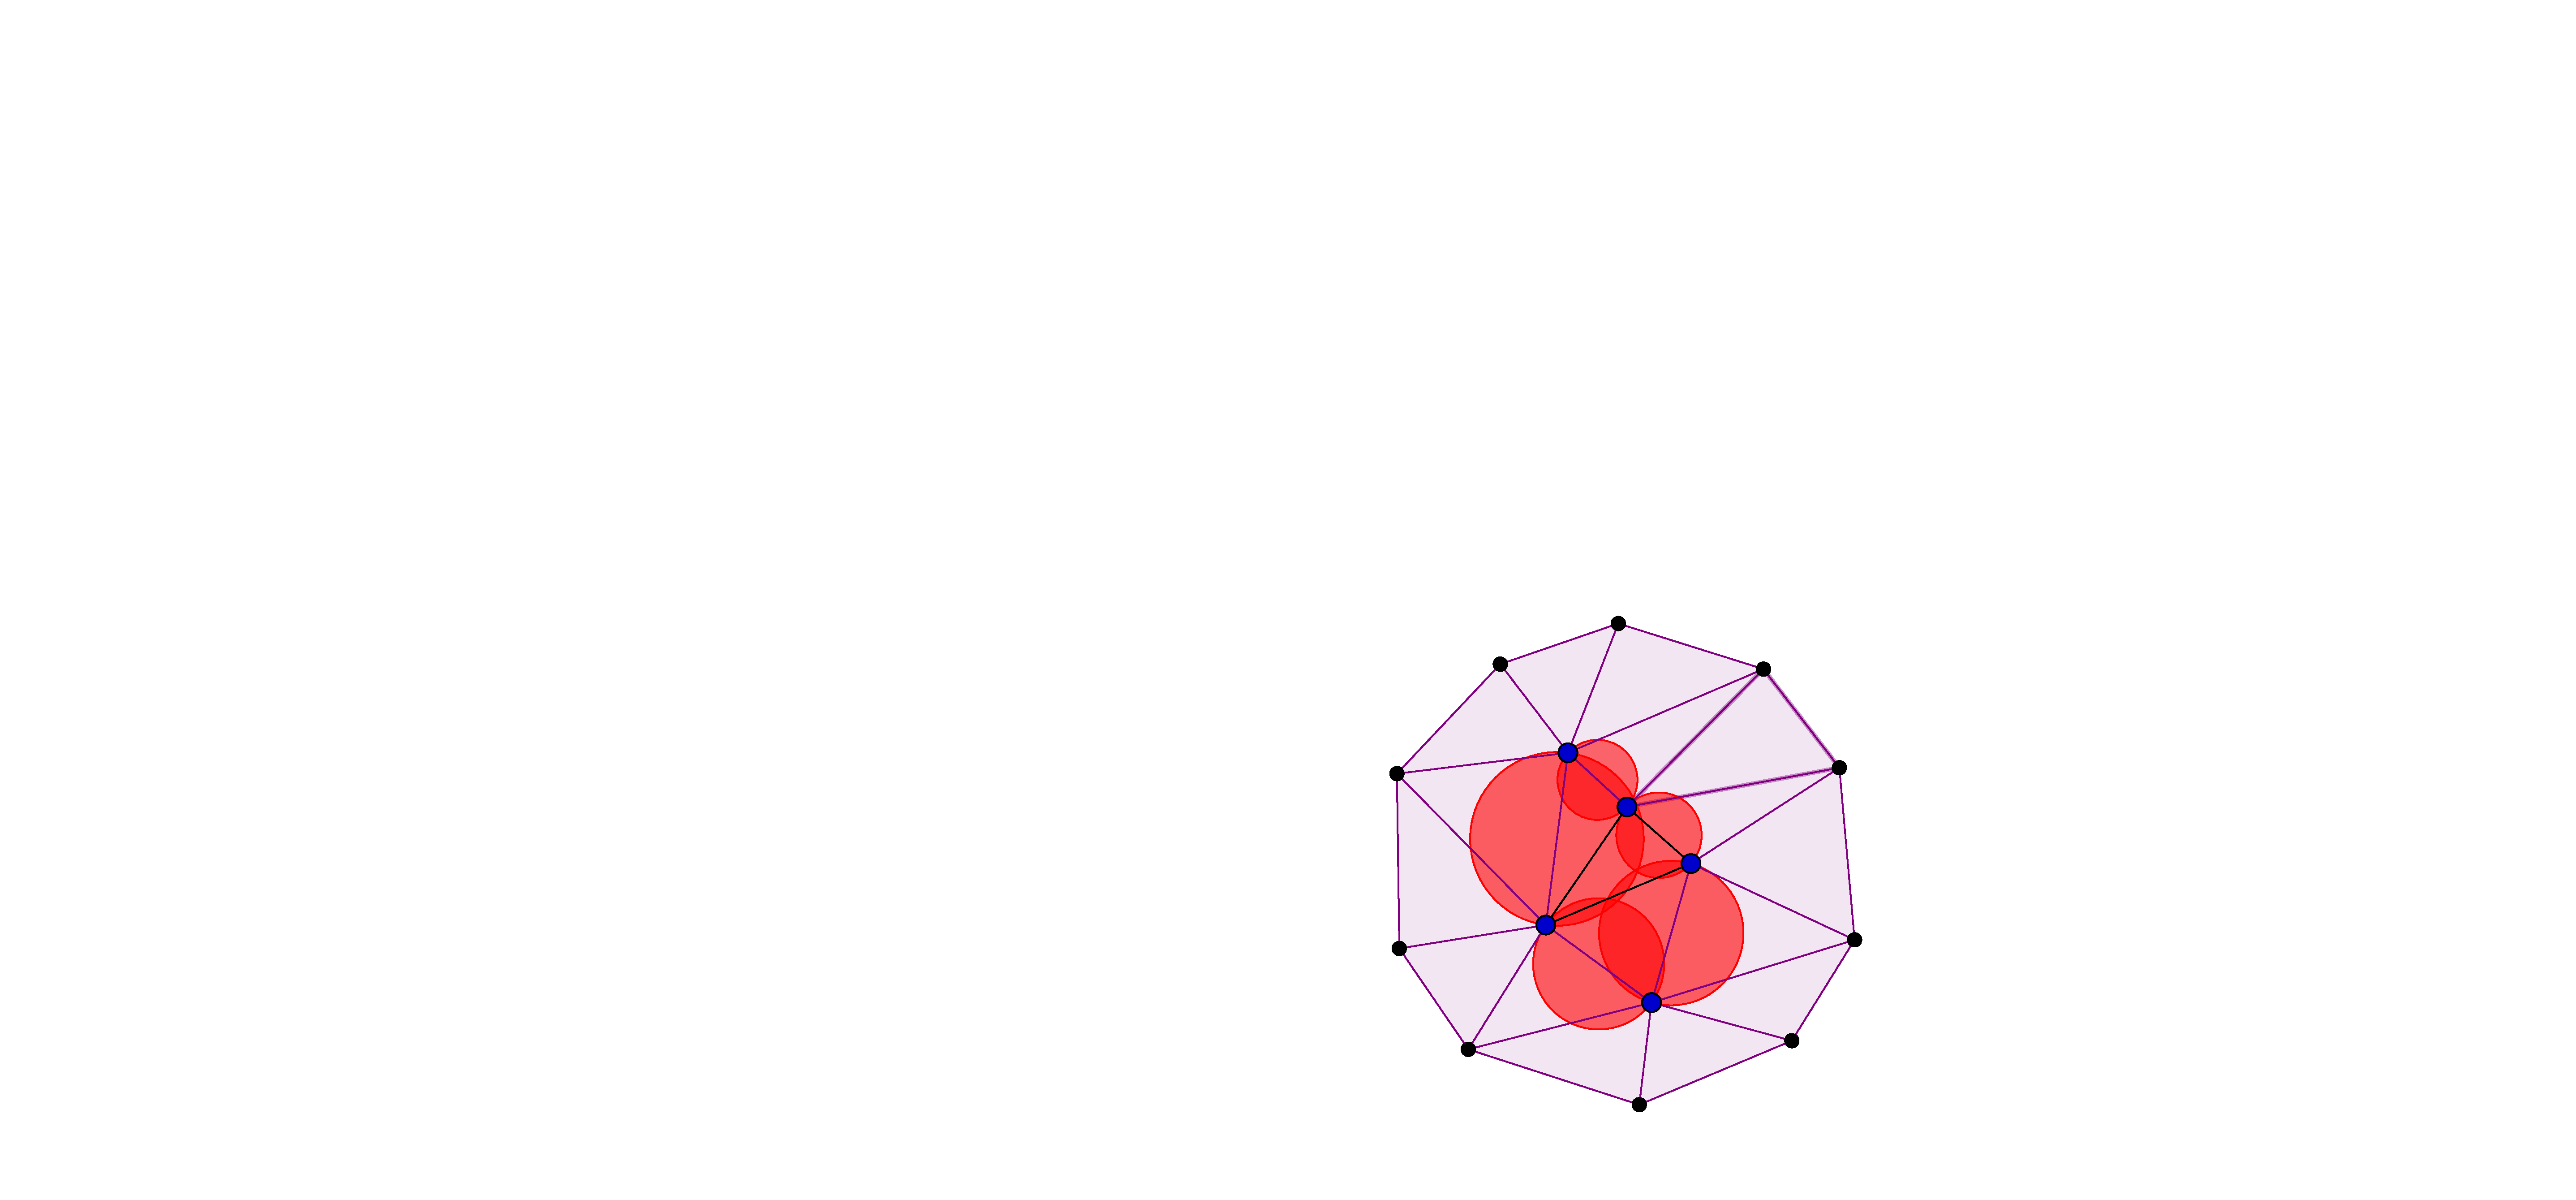
\includegraphics[width=4.0cm,height=4.0cm]{figs/operators/repel_a.pdf}
	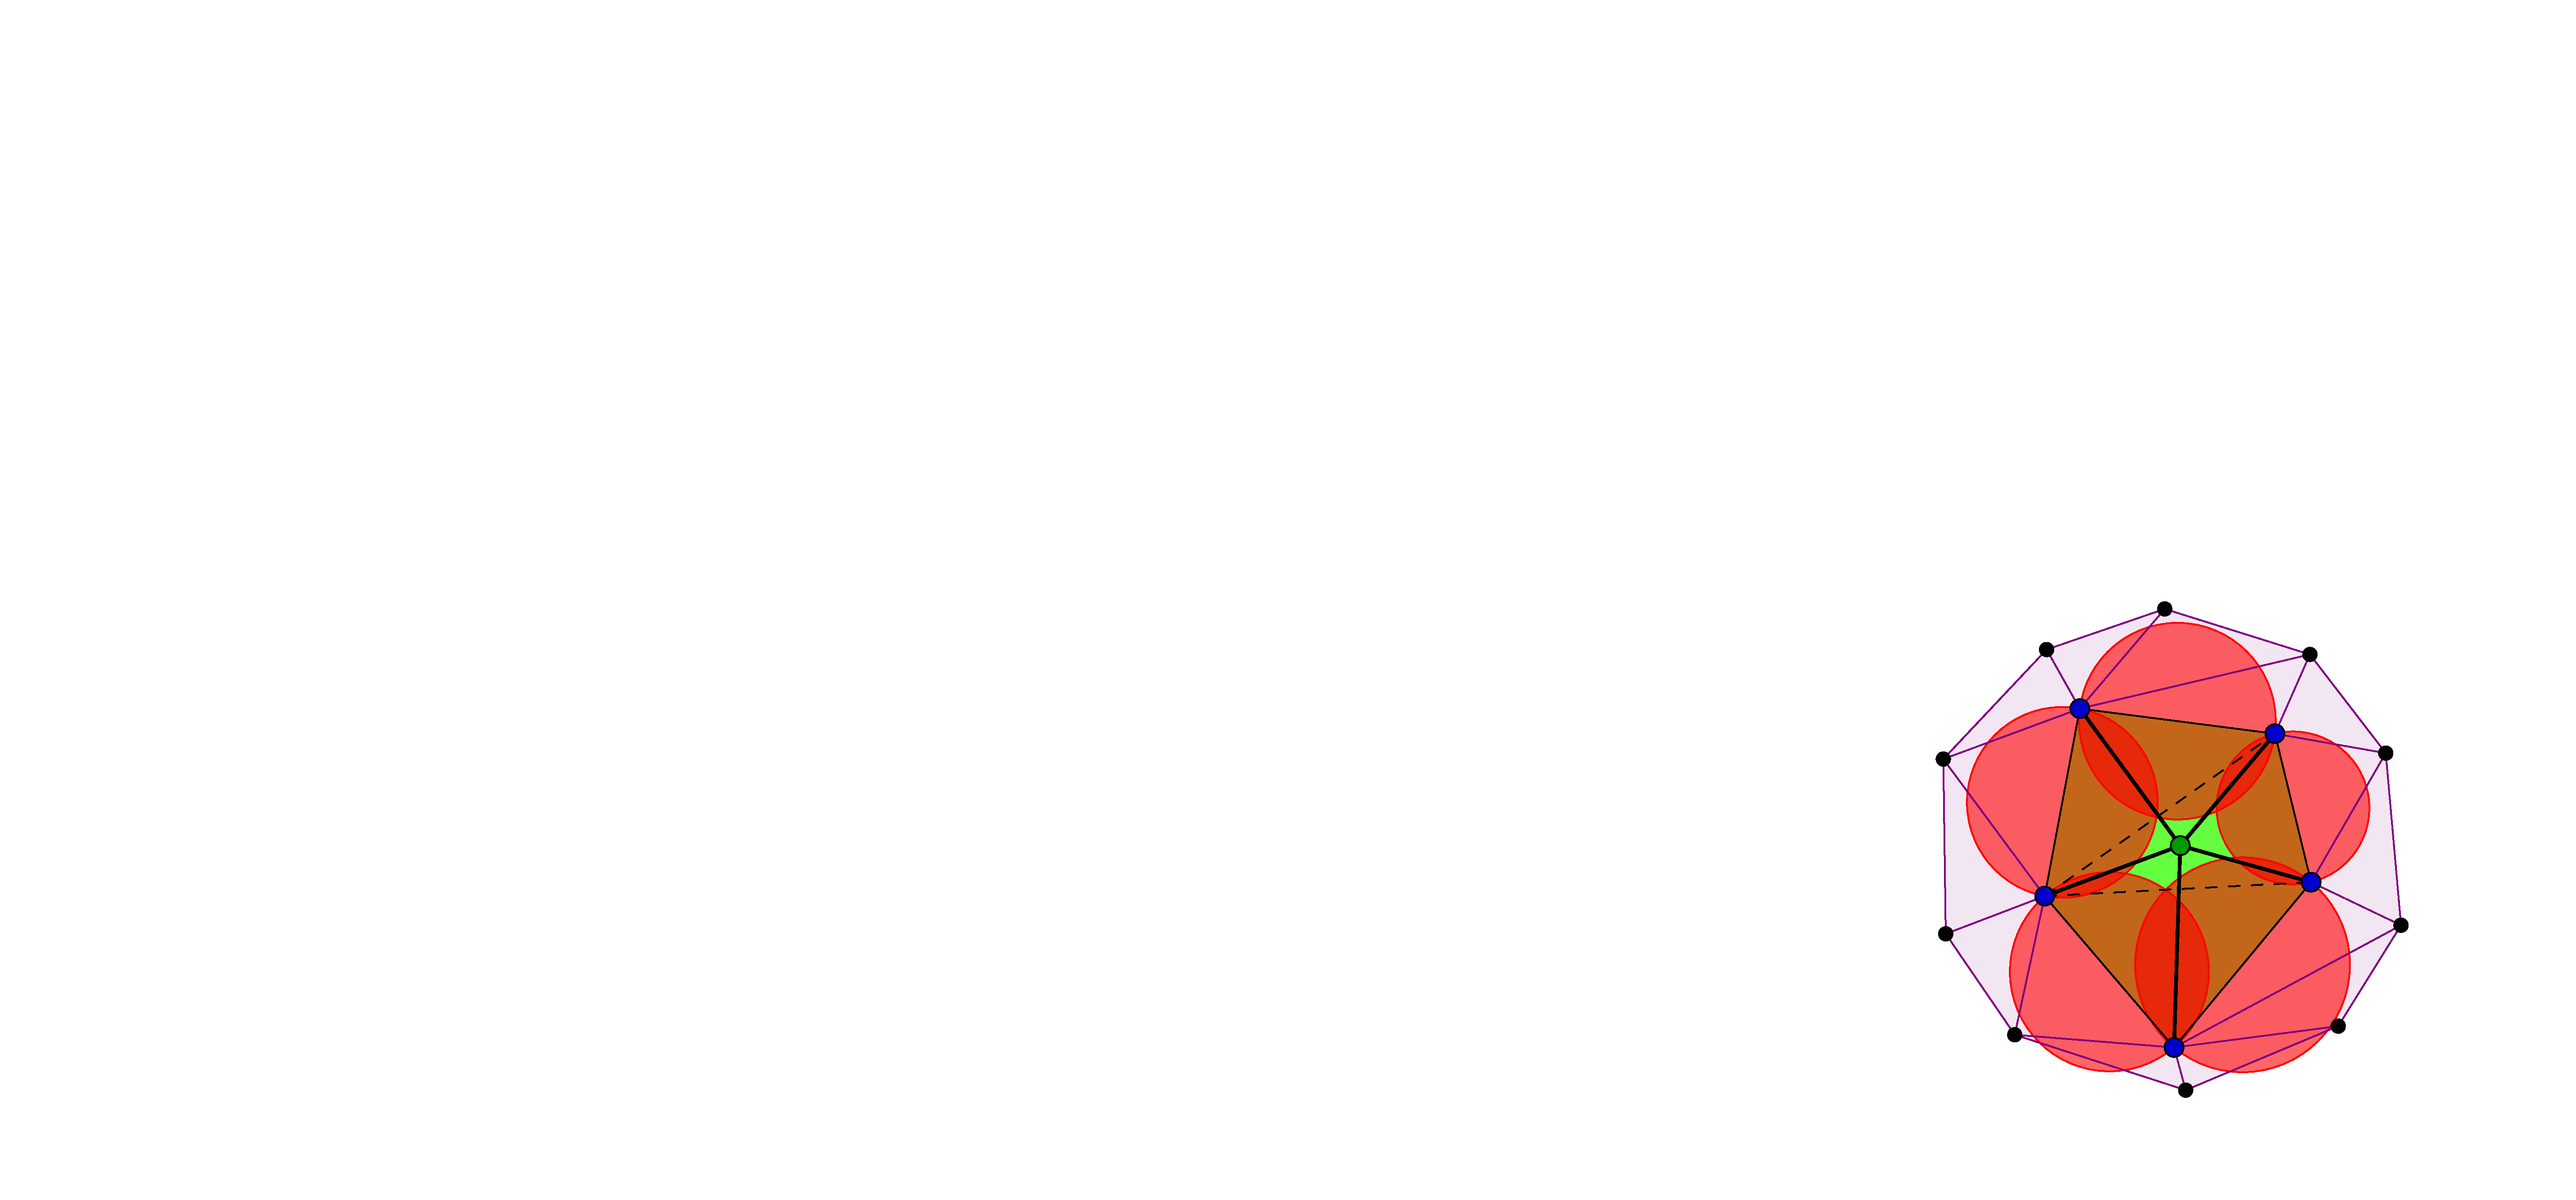
\includegraphics[width=4.0cm,height=4.0cm]{figs/operators/repel_b.pdf}
	}
	 %\caption{Resampling operators: replaced element(s) (crimson, dashed lines), bounding vertices (blue), new sample (dark green), inclusion regions (light green), exclusion regions (pink).}
	\caption{Sampling operators: red disks are exclusion regions; light green disks/polygons are inclusion regions; dotted lines and dark red vertices are the removed elements and vertices; thick dark lines and dark green vertices are the new elements and vertices; blue are the neighbor vertices. (a) Relocation of a vertex from the exclusion region to the feasible region. (b) Ejection of two vertices, one of which is associated with a bad element. (c) Injection of a new vertex. A low quality (red-ish) triangle is destroyed along with two other triangles such that the new vertex is not irregular (3-valent/4-valent). (d) Attractor Ejection where the intersection of inclusion disks is empty; relocating the neighbor vertices towards the ejected vertices to pack a feasible region. (e) Repeller Injection of new vertex where the exclusion disks cover the void completely; relocating the neighbor vertices farther away from the void creates a feasible region.}
	\label{fig:operators}
\end{figure*}

\begin{figure}[htb]
	\centering
	\subfloat[Nonobtuse.]{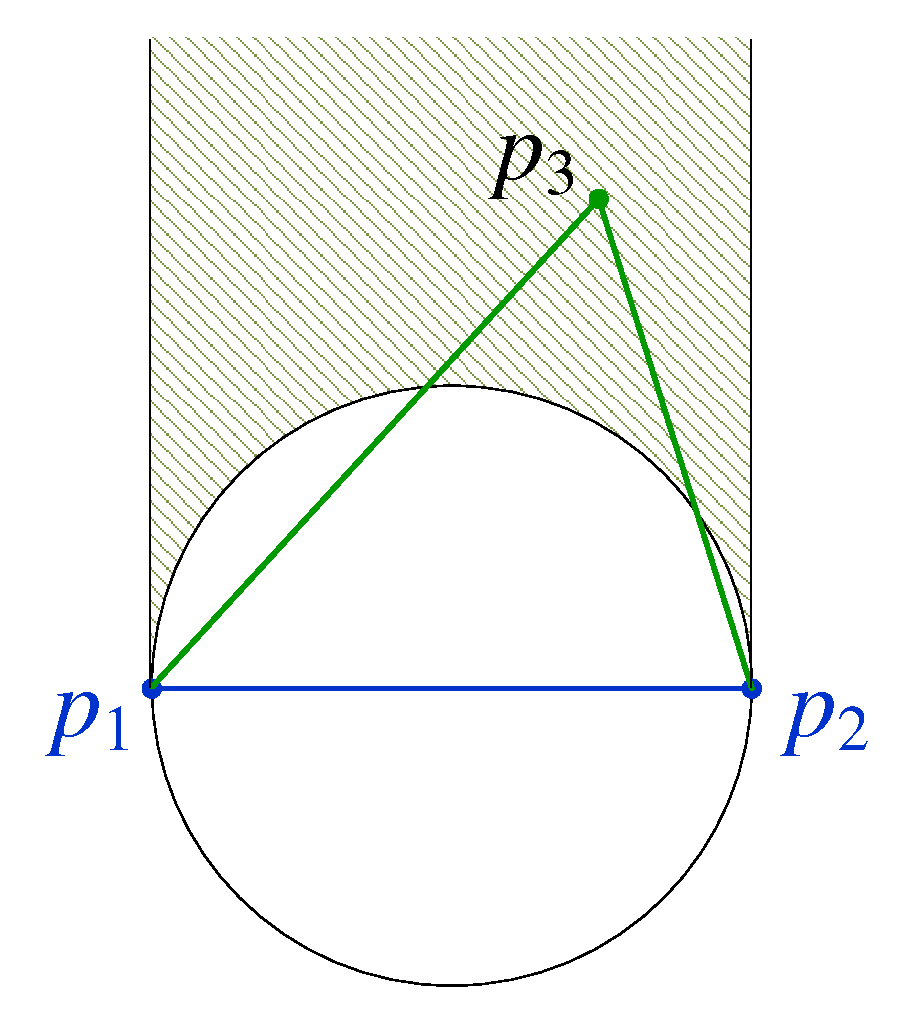
\includegraphics[width=0.25\columnwidth]{figs/regions1.pdf}}
	\quad
	\subfloat[$\protect\angle p_i \ge \theta_{\min}$.]{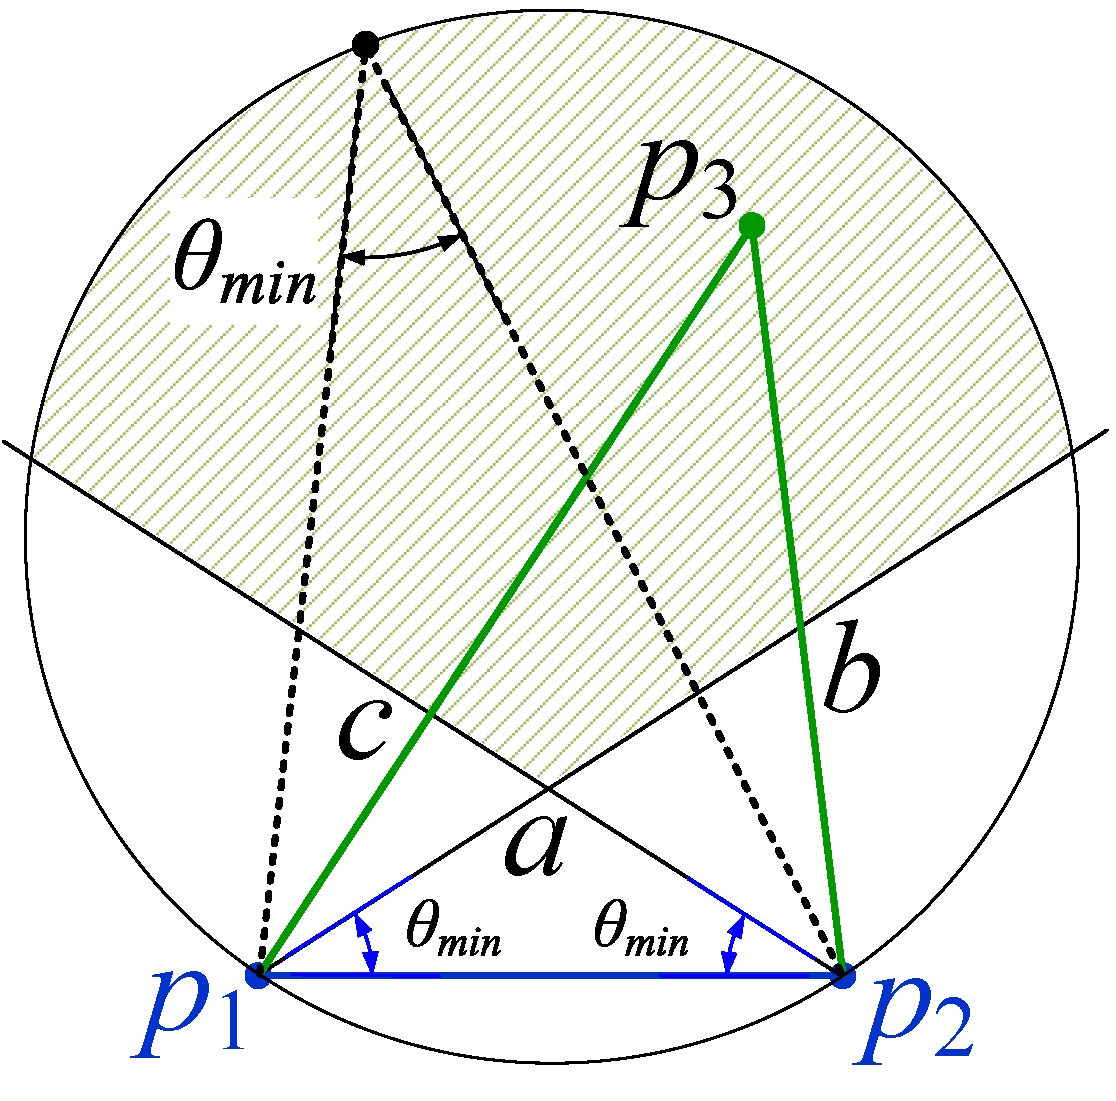
\includegraphics[width=0.25\columnwidth]{figs/regions2.png}}
	\quad
	\subfloat[Both objectives.]{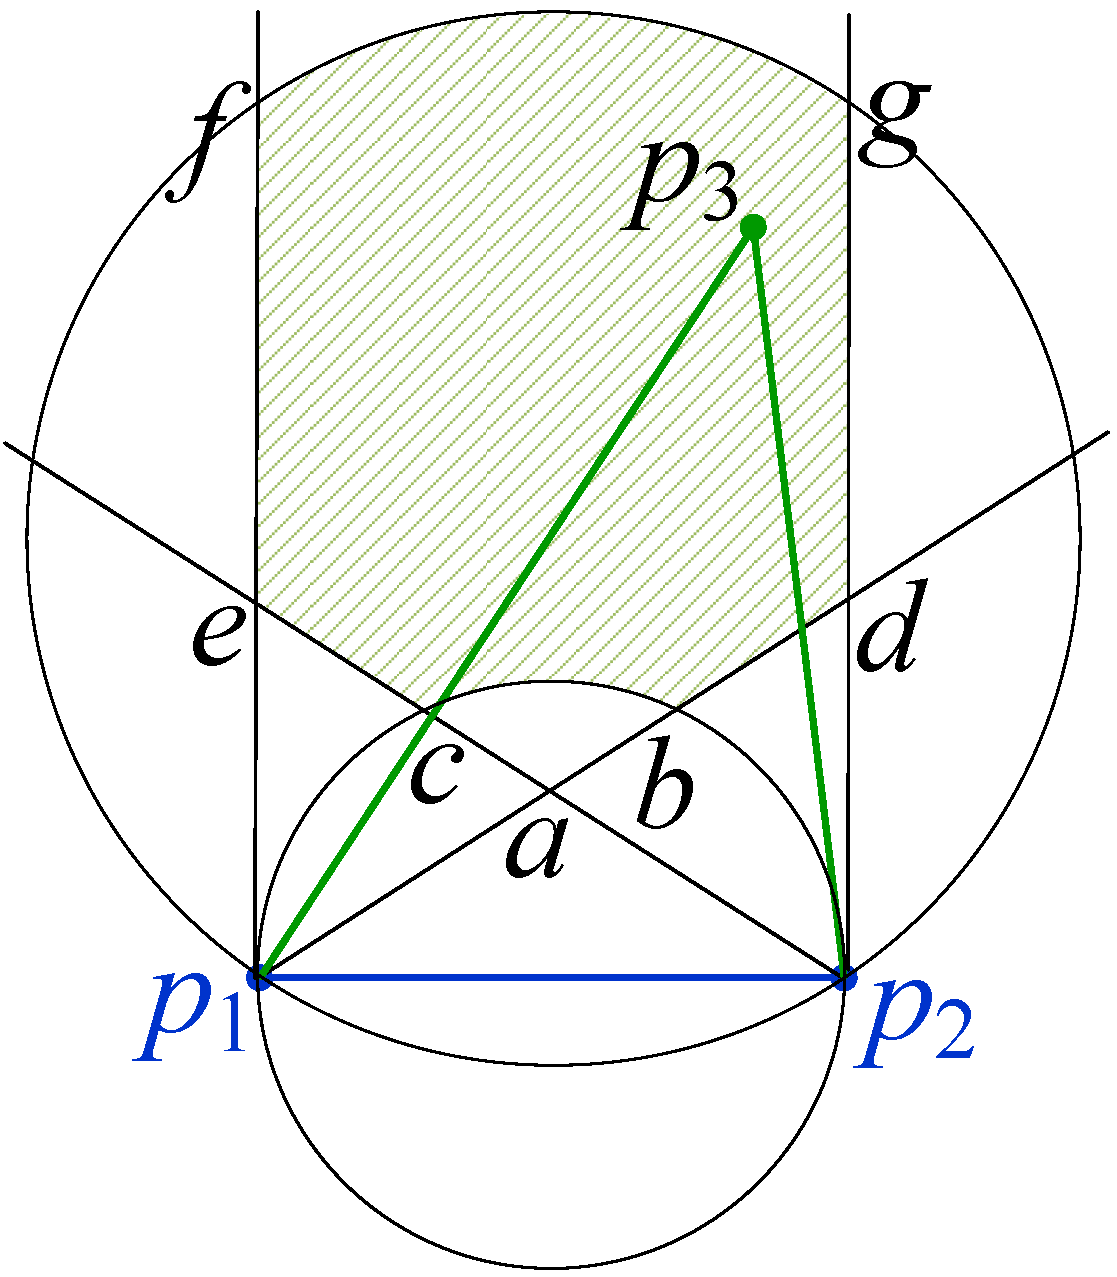
\includegraphics[width=0.25\columnwidth]{figs/regions3.png}}	
	\caption{Example primitives for resampling $p_3$ to form $\triangle p_1 p_2 p_3$: inclusion regions (green), exclusion regions (black boundaries).}
	\label{fig:regions}
\end{figure}

We notice that all operators seek monotonic improvement and do not allow degradation. This is a key feature that does not hold in previous art. 

\section{Reinforcement Learning Formulation:}
Here we extend the algorithm described above and formulate the problem as MDP problem. The algorithm contains all the important elements needed to improve an input mesh but lacks a coherent scheduling of the operators. The algorithm in the present form seeks to apply the operators with lowest magnitude of change i.e., Relocation and keep trying more aggressive operators at the end. Since it is not possible to fully understand the function being optimized, we turn to reinforcement learning as an aid to help choose a better scheduling.

The environment here is presented by the mesh vertices, current number of obtuse-triangles, and ratio of failed to successful attempts for each operator. These three parameters are enough to  described the current state of the environment and there is no need to trace the history of the vertices movement. That way, the problem can be treated as MDP problem. The agent goal is reduce the number of obtuse triangles through taking one action at a time represented by one of the remeshing operators. The problem is treated as an episodic tasks through which the agent trying to reach the optimal policy. 

For each action taken, it is successful in eliminate at least one obtuse triangle, we give a reward of one. Otherwise, the reward is always zero. We first experimented with giving negative rewards (-1) but this made the reward always negative. This could probably have some relation tied to the geometry of the problem. When final episode is represented by reaching non-obtuse mesh in which case a reward of 100 is given. If after number of episodes proportional to the number of initial mesh vertices is reached without reaching non-obtuse mesh, we give a reward of -100 and re-initialize the mesh. 


\section{Numerical Results:}
We applied several reinforcement learning algorithm over the stated problem. The algorithm were built on top of LibPGRL \citep{libpgrl} which fleixible implementation of several reinforcement learning application using C++. We experimented the above model using the following algorithms:
\begin{itemize}
\item Actor Critic with NeuralNet approximator
\item SARSA with NeuralNet approximator and Softmax policy with decaying temperature
\item SARSA with NeuralNet approximator and e-Greedy policy with constant epsilon
\item SARSA with NeuralNet approximator and e-Greedy policy with decaying epsilon
\item QLearning with NeuralNet approximator and Softmax policy with decaying temperature
\item QLearning with NeuralNet approximator and e-Greedy policy with constant epsilon
\item QLearning with NeuralNet approximator and e-Greedy policy with decaying epsilon
\end{itemize}
\section{Conclusion:}
For each algorithm, a run consisted of 1M steps which are averaged over 20 runs. For consistency over all algorithms, we used $\lambda=0.9$, $\kappa=10^{-4}$, $\epsilon=0.5$. We reached this values through experimenting with different values and tuning up and down. 

%\begin{figure}[tbh]
 %\centering     
 %  \subfloat [Bunny]{\includegraphics[width=0.24\textwidth]{bunny.png}}
 %  \subfloat [Fertility]{\includegraphics[width=0.24\textwidth]{fertility.png}}
 %  \subfloat [Sphere]{\includegraphics[width=0.24\textwidth]{sphere.png}}   
  % \subfloat [Torus]{\includegraphics[width=0.24\textwidth]{donut.png}}
   
  %   \caption{Results of brute-force ray tracing}
  % \label{fig:brute}
%\end{figure} 
   
 
\medskip

\bibliography{sample}

\end{document}
